We can generate a new world, with different terrain and placement of bushes, trees, forests and volcano. A world with 0.5 vertex density takes about 23 ms on a single 3.4 GHz Intel i5 core, which is fairly fast. The world looks very nice both close, however with tesselation even more so, and both far and very far away. An example of a world seen from far above is shown in figure \ref{fig:worldFromFarAbove}. The forests and the nature look really good compared to many games. It is a very fine foundation to build a game on, either a FPS or even a RTS or RPG, since it looks good at all ranges and the world can be big enough. With further work such as LOD levels for the vegetation and tesselation for the land, even vaster and richer worlds could easily be made.
\begin{figure}[H]
  \centering
  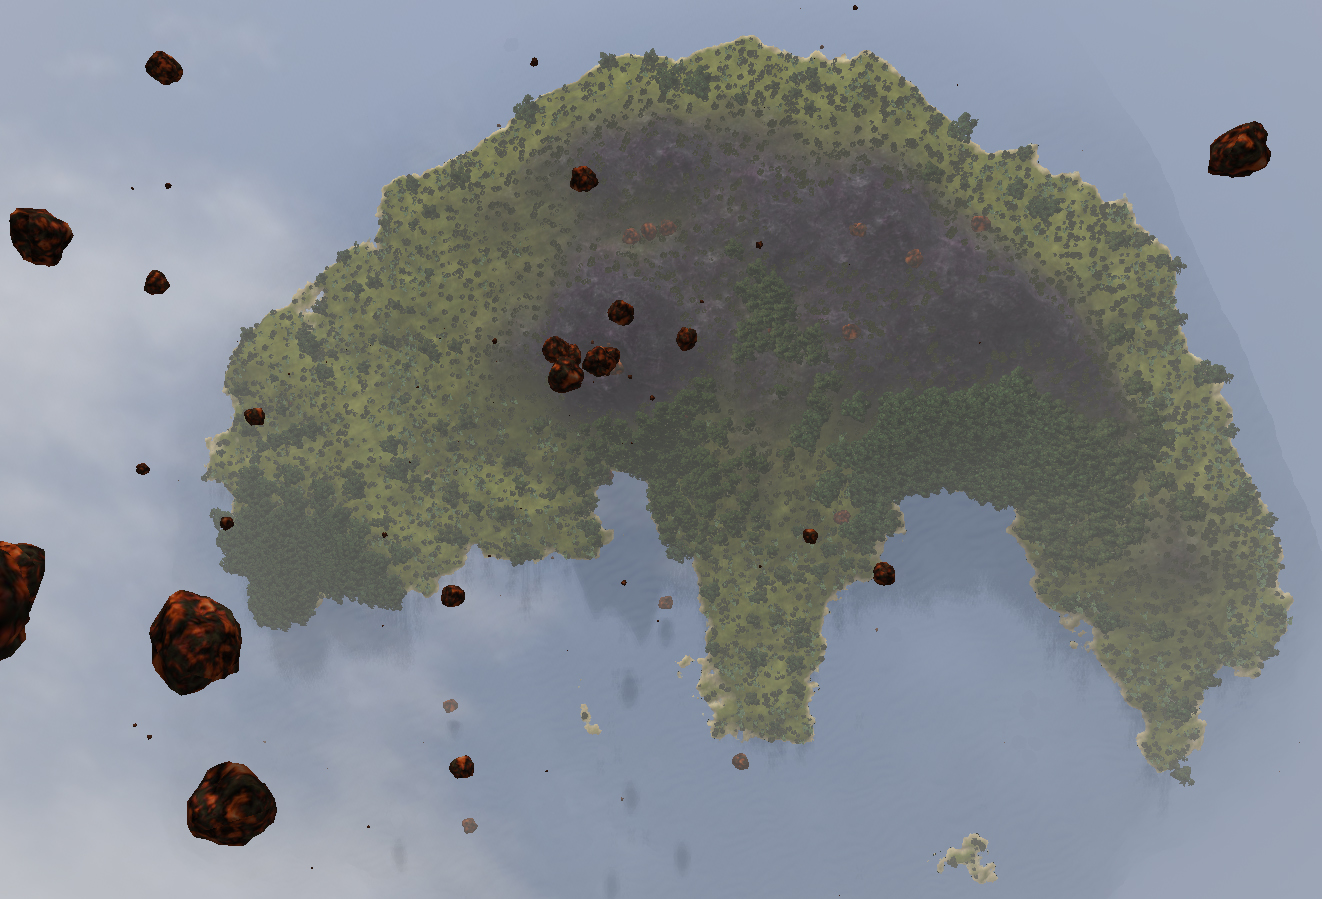
\includegraphics[width=\linewidth]{images/worldFromAFarTop.jpg}
  \caption{The final world from far above.}
  \label{fig:worldFromFarAbove}
\end{figure}%

Possible improvements and further work are Level Of Detail (LOD) objects for the vegetation, so that we can have even more vegetation, especially on low-end machines. Tesselation for the terrain is another thing that would make our world look much better and still work on slower machines. Living water with real waves could be accomplished if we use tesselation on a mesh grid, something we cannot afford right now without losing too much performance. The collision detection would allow for many more objects if we use an occree to segment the world. This would also be useful for an AI in any game/simulation that want to sense the close environment. Finally we lack some inhabitants to make use of our beautiful world and to bring it to live.
















